\section{Обзор существующих моделей паники}
\label{sec:overview}

В данном разделе будет произведен подробный обзор существующей научной литературы на тему моделирования массовой паники и сценария эвакуации.

\subsection{Работы Д. Хелбинга, П. Молнара, И. Фаркаса и Т. Вичека}
\label{sub:overview:helbing}

Данный пункт посвящен рассмотрению двух работ:

\begin{itemize}
  \item Simulating dynamical features of escape panic за авторством Д. Хелбинга, И. Фаркаса и Т. Вичека~\cite{helbing_escape_panic};
  \item Simulation of pedestrian crowds in normal and evacuation situations за авторством Д. Хелбинга, И. Фаркаса, П. Молнара и Т. Вичека~\cite{helbing_evacuation}.
\end{itemize}

Эти две работы рассматриваются вместе, так как высказывают очень похожие идеи.
Вторая статья (Simulation of pedestrian crowds in normal and evacuation situations) по сути является развитием и обобщением предыдущей работы данного коллектива,
а также нескольких других статей Д. Хелбинга.

Статья концентрируется на рассмотрении массовых мероприятий и больших скоплений людей (толп).
Выделяются два различных сценария поведения: нормальный сценарий и сценарий массовой паники.
На основе множества социальных и психологических исследований, выделяются следующие отличия поведения людей в сценарии массовой паники по сравнению с нормальным сценарием:

\begin{itemize}
  \item люди становятся более нервными, то есть быстрее и чаще принимают необоснованные решения;
  \item люди стараются двигаться значительно быстрее чем обычно;
  \item люди начинают толкаться, взаимодействия между людьми становятся физическими по природе;
  \item движение в целом и проход через узкие места в частности становятся нескоординированными;
  \item на выходах наблюдаются скопления людей;
  \item физические взаимодействия внутри толпы складываются: суммарное давление может составлять до 4500 $\text{Н} / \text{м}^2$,
        что достаточно для разрушения кирпичных стен и повреждения стальных конструкций;
  \item движение затруднено упавшими и ранеными людьми, которые становятся <<препятствиями>>;
  \item люди демонстрируют <<стадное поведение>>, то есть делают то же, что и другие люди вокруг них;
  \item люди часто не замечают запасные выходы, запасные выходы в целом используются неэффективно.
\end{itemize}

Далее авторы статьи отмечают, что хотя поведение толп людей имеет множество аналогий с потоками газов (жидкостей), данные аналогии не совсем хорошо работают в сценарии массовой паники.
Вместо использования газо-кинетической модели, авторы предлагают воспользоваться разработанной ими моделью социальных сил.
Более подробно данный вопрос был рассмотрен в дипломном проекте~\cite{my_diploma}, поэтому здесь будет представлена краткая справка о различных моделях поведения толпы.

Исторически одними из первых моделей поведения толпы были газокинетические модели, которые использовались для моделирования транспорта.
Они представляют собой попытки применить множество аналогий, имеющихся между потоком пешеходов и потоком газа (жидкости).
Газокинетические модели являются макроскопическими моделями "--- это означает, что объектом моделирования является поток пешеходов, а не каждый отдельный пешеход.
В отличие от макроскопической модели, в микроскопической модели объектом моделирования является каждый отдельных пешеход,
а интересующие нас характеристики получаются методом аггрегации множества параметров отдельных пешеходов.
Микроскопические модели намного более гибкие чем макроскопические модели, и показывают более высокую точность предсказаний.
Таким образом, авторы указывают на несостоятельность использования макроскопических моделей в сценарии массовой паники, и предлагают собственную микроскопическую модель.

Авторы кратко описывают базовую модель социальных сил в простом варианте с двумя силами "--- силой притяжения к цели и силой отталкивания от препятствий.
Подробное описание данных концепций можно найти в уже упомянутом дипломном проекте.
Далее, авторы вводят новую силу для представления физических взаимодействий между людьми.
Данная сила похожа на силу отталкивания, имеет несколько ключевых отличий:

\begin{itemize}
  \item применяется только при условии физического контакта между двумя людьми;
  \item имеет два компонента: прямое отталкивание от контакта и аналог силы трения, препятствующий тангенциальному движению.
\end{itemize}

Также авторы вводят линию распространения огня, используя для этого обычную отталкивающую силу с повышающим коэффициентом.

В результате авторы с помощью разработанной модели получили множество интересных результатов, включая самоорганизующиеся потоки людей в обычном сценарии,
уменьшение потока людей на выходе при наличии комбинации расширения и сужения пространства, и др.

\begin{figure}[ht!]
  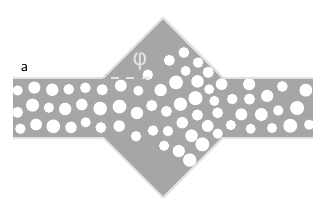
\includegraphics[width=\dimexpr\linewidth-13em\relax]{helbing_sim_example}
  \caption{Пример одной из симуляций в обсуждаемой работе}
  \label{sub:overview:helbing:sim_example}
\end{figure}

Пример одной из симуляций (с комбинацией расширения и сужения доступного пространства) можно увидеть на рисунке~\ref{sub:overview:helbing:sim_example}.


\subsection{Модель А. Кирчнера и А. Шадшнейдера на основе клеточного автомата}
\label{sub:overview:kirchner}

Предлагаемая авторами в работе Simulation of evacuation processes using a bionics-inspired cellular automaton model for pedestrian dynamics~\cite{kirchner2002simulation} модель представляет собой интересную вариацию модели клеточного автомата.

Модель клеточного автомата "--- модель с дискретным пространством и определенными правилами движения по нему.
Дискретное пространство представляет собой набор клеток. Каждый пешеход занимает одну клетку.
Правила движения представляют собой набор условий, по которым пешеход переходит из своей текущей клетки в одну из соседних.

Авторы отмечают, что их разработка основывается на аналогии с биологическим процессом хемотаксиса и поведением некоторых насекомых.

Хемотаксис "--- это двигательная реакция организмов (чаще всего простейших) на химический раздражитель.
При этом химические раздражители подразделяются на аттракторы и репелленты.
Соответственно, организм движется по возрастающему градиенту аттрактора и наоборот, по убывающему градиенту репеллента.

Поведение некоторых насекомых, на которое ссылаются авторы, заключается в следующем:
каждая особь оставляет за собой некий химический след, который могут обнаружить другие особи.
В случае, если особь находит источник еды, данный химический след усиливается.
Для других особей сильный химический след является аттрактором, что приводит к определенной форме кооперации "---
набор особей более эффективно находит источники еды (по сравнению с индивидуальным поведением).

Людям свойственны намного более сложные механизмы кооперации, однако описанный механизм может служить простой моделью человеческого поведения в стрессовой ситуации,
когда сложные механизмы не используются. По мнению авторов, данный <<след>> может представлять собой некое абстрактное отображение маршрута, известного пешеходам,
а механизм накопления является аналогией следования за людьми, уже идущими по нужному маршруту.

Для реализации данной модели в рамках клеточного автомата авторы ввели два <<химических>> поля "--- статическое и динамическое.
В данном случае поле представляет собой дискретную функцию, ставящую в соответствие каждой ячейке некоторое значение.
Положительное значение представляет собой аттрактор, а отрицательное "--- репеллент.
При этом статическое поле не меняется в пределах одного запуска симуляции и представляет собой описание окружения,
где выходы являются аттракторами, а источники опасности "--- репеллентами.
Динамическое же поле используется для создания <<химического>> следа.

В рамках модели клеточного автомата в качестве правил движения было выбрано правило хемотаксиса "---
движение в строну возрастающего градиента аттрактора и наоборот, в сторону убывающего градиента репеллента.

Своей целью авторы ставят исследование различных типов поведения в стрессовых условиях.
И хотя предложенная модель на первый взгляд кажется немного странной, авторы смогли получить те же результаты,
что и другие исследователи с намного более сложными моделями (в частности, в рамках зависимости времени эвакуации от <<стадного>> поведения).
Однако в отличие от других моделей, данная модель очень проста в реализации и эффективна, что позволяет использовать ее для симуляции большего числа людей.

\begin{figure}[ht!]
  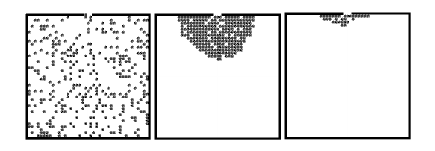
\includegraphics[width=\dimexpr\linewidth-9em\relax]{kirchner_sim_example}
  \caption{Пример одной из симуляций в обсуждаемой работе. Слева "--- изначальное положение (t = 0). Посередине "--- промежуточное положение. Справа "--- заключительная стадия (осталось всего несколько частиц)}
  \label{sub:overview:kirchner:sim_example}
\end{figure}

Пример одной из симуляций (с наблюдаемым эффектом скопления у выхода) можно увидеть на рисунке~\ref{sub:overview:kirchner:sim_example}.

\subsection{Агентное моделирование}
\label{sub:overview:agent}

Рассмотрим агентное моделирование на основе работы Agent-Based Modeling and Simulation on Emergency Evacuation~\cite{ren2009agent} за авторством Ч. Рена, Ч. Янга и С. Джина.

Данная работа предлагает следующую классификацию имитационных моделей:

\begin{itemize}
  \item имитационные модели дискретных событий;
  \item имитационные модели динамики систем;
  \item имитационные модели на основе агентов.
\end{itemize}

Имитационные модели динамики систем обычно являются макроскопическими моделями, представляющими параметры системы как некоторую функцию от времени и других параметров системы.

Имитационные модели дискретных событий обычно оперируют дискретным временем, меняя состояние системы по определенным событиям.

И наконец имитационные системы на основе агентов представляют собой микроскопические модели,
где каждый объект моделирования (<<агент>>) принимает собственные решения на основе состояния системы и параметров других агентов.
При этом правила поведения агентов должны быть достаточно простыми, а объектом исследования является то, как набор простых правил
вызывает сложные макроскопические эффекты в системе.
Как можно заметить, модель рассмотренная в разделе \ref{sub:overview:helbing} по данной классификации является имитационной моделью на основе агентов.

Далее авторы описывают свою модель на основе агентов, разработанную в среде моделирования Repast.
Данная модель концентрируется на индивидуальных параметрах классов пешеходов и их влиянии на время эвакуации.
Например, данная модель подразделяет всех участвующих пешеходов на женщин, мужчин и детей, при этом каждый класс имеет свой набор параметров.
Также в модель введены параметры <<лидерства>> и <<независимости>>, задающие соответственно желание вести других людей за собой и желание следовать за лидером.

Авторы исследуют зависимости времени эвакуации от набора параметров, таких как наличие и качество <<лидеров>> и др.
Результаты авторов совпадают с другими моделями, и может считаться их подтверждением.

Более интересным применением агентного моделирования является работа Detection of primitive collective behaviours in a crowd panic simulation based on multi-agent approach~\cite{patrix2012detection} за авторством Дж. Патрикса, А. Моуаддиба и С. Гейтпейла.

В данной работе агенты действуют в соответствии с двумя разными типами поведения, и переключаются между ними в зависимости от внешних условий.
Первый тип поведения "--- реакция (рефлекс) на некоторую рискованную ситуацию "--- возникает как непосредственный ответ на внешний стимул.
Второй тип поведения "--- сознательный "--- отвечает за долгосрочное планирование.

Так же как и авторы клеточной модели, описанной в разделе \ref{sub:overview:kirchner}, для описания коллективного поведения авторы обращаются к аналогиями из мира биологии,
в частности к тому же <<химическому>> следу феромонов муравьев и поведению стаи птиц.
Например, поведение каждой особи в стае может быть описано следующими правилами:

\begin{itemize}
  \item правило разделения: особи пытаются избежать столкновения с ближайшими особями;
  \item правило равнения: особи пытаются лететь в том же направлении, что и ближайшие особи;
  \item правило сплоченности: особи пытаются держаться недалеко от ближайших особей.
\end{itemize}

На основе всех описанных правил и типов поведения авторы строят сложную модель поведения агента.
Однако, это не является конечной целью исследования "--- авторы хотят получить возможность детектировать интересующие паттерны поведения в толпе.
Для этого авторы представили все возможные изменения внутреннего состояния агента как случайное событие, и составили цепь Маркова из этих случайных событий.
С помощью методов машинного обучения, используя последние несколько звеньев цепи Маркова, авторы пытаются детектировать определенные паттерны поведения.

Результаты данной работы включают в себя факты детектирования возникновения паники и очагов опасности, а так же успешных симуляций сложных систем.

\begin{figure}[ht!]
  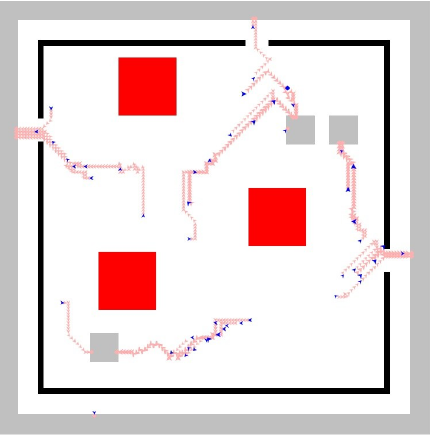
\includegraphics[width=\dimexpr\linewidth-5em\relax]{patrics_sim_example}
  \caption{Пример одной из симуляций в обсуждаемой работе. Предсказание поведения агентов в условиях паники}
  \label{sub:overview:patrics:sim_example}
\end{figure}

Пример одной из симуляций (с предсказанием поведения в условиях паники с помощью машинного обучения) можно увидеть на рисунке~\ref{sub:overview:patrics:sim_example}.


\subsection{Социологические и психологические исследования}
\label{sub:overview:soc}

Следует отдельно отметить множество социологических и психологический исследований паники \cite{mawson2005understanding}~\cite{quarantelli1975panic}~\cite{quarantelli2001sociology}~\cite{quarantelli1979panic}.

Хотя к теме моделирования паники они явно не относятся, благодаря им и набору эмпирических наблюдений были выявлены особенности панического поведения,
которые затем могут быть применены при моделировании паники.


\subsection{Расчетная модель по ГОСТ 12.1.004-91}
\label{sub:overview:gost}

На территории Республики Беларусь действует ГОСТ 12.1.004-91 <<Система стандартов безопасности труда. Пожарная безопасность. Общие требования>>~\cite{gost_fire_safety},
определяющий требования пожарной безопасности к зданиям.

Также данный ГОСТ определяет требования к времени эвакуации из здания, предоставляя расчетную модель для вычисления фактического времени эвакуации.
Данная модель описана отдельно в рекомендации по расчету параметров эвакуации людей на основании положений ГОСТ 12.1.004-91 ''Пожарная безопасность. Общие требования''~\cite{model_gost}.

Расчетная модель сводится к разбиению пути эвакуации на участки, определению самого длинного (<<диктующего>>) маршрута эвакуации, и расчет времени эвакуации по этому маршруту.
Суммарное время эвакуации принимается равным сумме времени эвакуации через каждый участок.
Время эвакуации через каждый участок зависит от его расчетной длины и ширины, а также расчетного потока через этот участок.
Если поток превышает некоторый пороговый поток, то ко времени дополнительно добавляется время задержки.

Данная модель зарекомендовала себя как достаточно точный способ вычисления времени эвакуации, и может быть использована для калибровки имитационных моделей.






